\subsection{PIMS Stats Module}
This module is responsible for displaying statistics from the database. The user has an option to choose the type of graph (either a bar chart or line graph). \par 

\subsubsection{Scope}
The scope is shown in the use case diagram below: \par
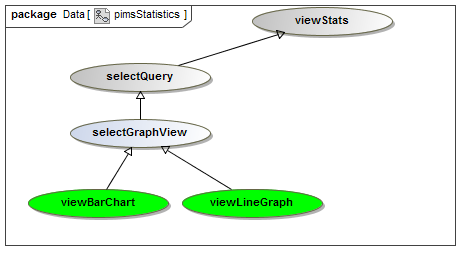
\includegraphics[width=\linewidth]{./Graphics/pimsStats/pimsStatistics}

\subsubsection{Use cases}
\begin{description}
	\item{\textbf{createGraph -- priority: critical}} This use case is meant to be used by the front-ends to create and display a graph. This graph can be viewed by the client  and the client can predict and print this data for record keeping.
	\begin{description}
		\item{\textbf{Service Contract}} The service contract for createGraph is shown below. It is a simple graph function.
		\begin{figure}[h!]
			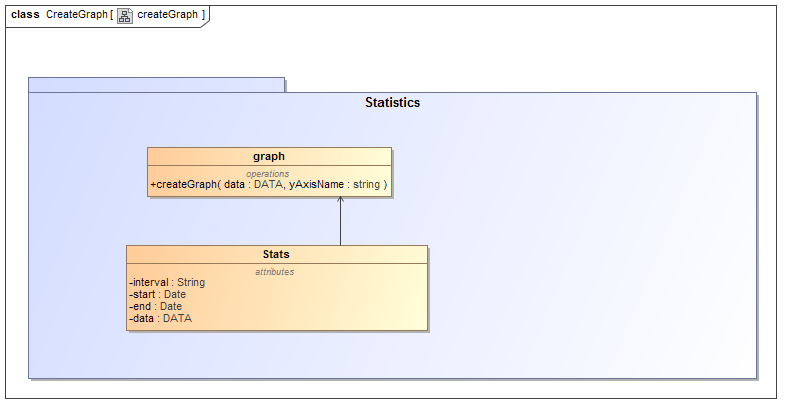
\includegraphics[width=\linewidth]{./Graphics/pimsStats/createGraph}
		\end{figure}
	\end{description}
	\item{\textbf{Stats -- priority: critical}} This use case is a generic version of all statistics to be obtained. All statistics will be shown in generic form to allow for simplicity and non-repetition of modules.
	\begin{description}
		\item{\textbf{Service Contract}} The generic service contract for all statistics is shown below. It is a simple statistics query:
		\begin{figure}[h!]
			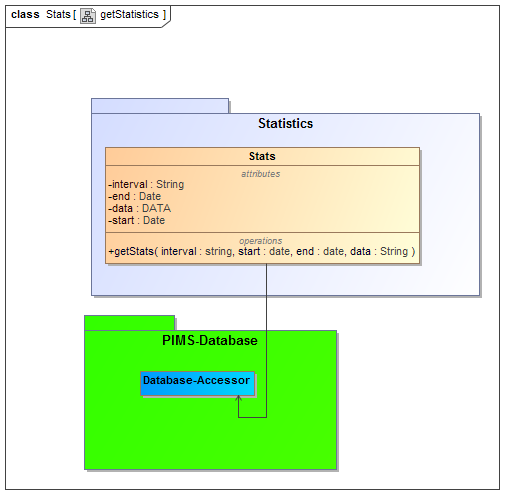
\includegraphics[width=0.5\linewidth]{./Graphics/pimsStats/getStatistics}
		\end{figure}
	\end{description}
\end{description}

\subsubsection{Equations}
\begin{description}
	\item{\textbf{Statistics Average Equation}}\hfill\\
		\(AM = \frac{1}{n}\displaystyle\sum_{i=1}^{n}\displaystyle\sum_{j=1}^{x} a_j \)
	\item{\textbf{Graph Equation}}\hfill\\
		\(f(x) = \displaystyle\sum_{i=1}^{n} x_i \)
\end{description}
